
\section{EMBEDDED LINUX - for me}


\subsection{Vid 0 - Build the image for Beaglebone Black}


\subsection{Vid 1 - Lam quen voi Linux}

warning level cua compiler should be set at the highest level, try to fix the warning.
\\co 2 cach de tim kiem 1 text trong linux, su dung grep hoac la su dung cscope, cscope thi thich hop voi nhung du an lon
\\co the setup visual studio code voi gdb va kernel de su dung cho thuan tien


\subsection{Vid 2 - Gioi thieu ve file, directory, multithread, user, etc. (Nov 11, 2021)}

02m: gioi thieu ve file, directory, multithread, user, etc.
\\04m:
\\ps - aux | grep hello - list all the process running in the pc, with the name hello
\\ls /proc/2821 - list all the files used in the process that has the id = 2821
\\ls -l /proc/2821/exe - show the directory of the execute file of the process id 2821, which is c02-hello
\\cat /proc/2821/maps - list all the libraries used in this process
\\cat /proc/2821/cmdline - list the command line used to call the execute file, which is "./c02-hello"
\\11m: the antivirus software detects the keylogger by checking the checksum of the binary files, so if you write your own keylogger cannot detect it until the checksum is updated into the antivirus software database.
\\16m: check all the files in the /proc/id-num to know more information about the process, ex.: could read how much ram, size of that process
\\20m: lap trinh voi file de doc ghi du lieu co ban
\\21m: 3 steps, step 1 > open file, step 2 > edit file, step 3: close the file. same as malloc.
\\good practise: write close file function right after open file function and then enter and write the code in the middle.
\\cach search: open() linux, them keyword linux vao trong phan search, va doc tu cac trang web cua hang viet ra linux, ex.: man7.org
\\31m: echo "hi everyone, minh la Hoang Ham Hoc" > data : write the content " hi everyone, minh la Hoang Ham Hoc " to the file named "data"
\\1h15m: checkpath and fix the homework - writing name into existed file
\\1h17m: fix loi DOS line ending, checkpath khac gi response tu gcc? -> follow linux kernel coding style (convention): kernel dot org coding style. 
\\checkpath co the check phan code ban them vao va ignore phan code cu ko co thay doi. (ex: check patch cua firmware, co the coi video tu 1h17 de lam theo)
\\fix loi ten xuong dong, lam sao de doc errno?
\\2h00m: cach debug ve struct khi open / close file.


\subsection{Vid 3 - Signal (Nov 13, 2021)}

use command "ps -aux | grep c03\_signal" to list the process id of the task name "c03\_signal"
\\use command "kill" to send signal, not kill the process, ex: kill -SIGUSR1 17748, then in the terminal will call the func. my\_handler, print out the value of the sig\_num
\\printf thuong se ghi du lieu vao stdout, doi khi printf se luu vao buffer, nhung phai co them 'sur n' thi no moi day ra ngoai man hinh 
\\trong che do console mode, ko co dau x de dong app, nen khi minh nhan Ctrl + C thi se terminate 1 cai app trong che do console mode.
\\Control + C se gui 1 cai signal toi cho app, gia tri cua signal do la SIGINT P1990, interrupt from keyboard, xem o man7.org.
\\1h10m: vi du ve dung to hop phim de gui 1 signal di, Ctrl + C interrupt from keyboard, Ctrl + Z quit the app. Cac signal nay chi gui den foreground cua Linux kernel, chu ko gui den background.
\\Signal co the gui kem du lieu (data) vao trong signal
\\Hoan thanh vi du, nhan "Ctrl + C" de inlog du lieu
\begin{itemize}
  \item Change the code of the signal from SIGUSR1 to SIGINT (interrupt from keyboard), search with keywords: signal linux
  \item then add the printf You have pressed Ctrl C in the my\_handler function.
  \item run the compiled code and press "Ctrl + C"
\end{itemize}

\begin{figure}[h]
  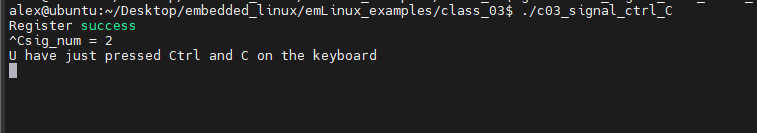
\includegraphics[scale=0.5]{emLinux_c03_signal_ctrl_C}
  \caption{The result of the example}  
\end{figure}



1h20m: phan quyen de chay process, moi cau lenh deu phai xem cai quyen cua minh o dau, day co the gay loi cho chuong trinh cua ban
\\1h27m: phai check sau moi cau lenh, de xem init co thanh cong hay ko, vd char *a = malloc, thi phai check if(NULL != a), neu ko co loi thi moi chay func cua minh
\\ngoai ra thi phai check errno (error number).
\\IMPORTANT: errno only stores the value of the latest process.
\\1h41m: co nhieu process qua thi dung kill -9 process\_id.
\\chu y vao trang thai cua process, T, R+, T means terminated 
\begin{figure}[h]
  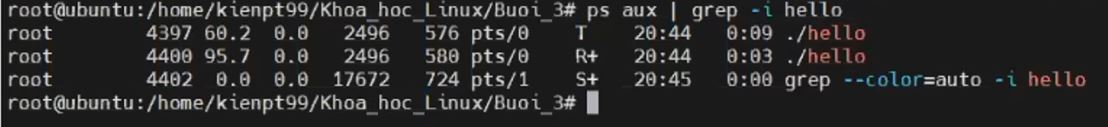
\includegraphics[scale=0.5]{emLinux_c03_multiple_processes}
  \caption{Multiple processes but different status - stop T, running R}  
\end{figure}

google keyword /proc/stat linux from man7.org for more information about the process
\begin{figure}[h]
  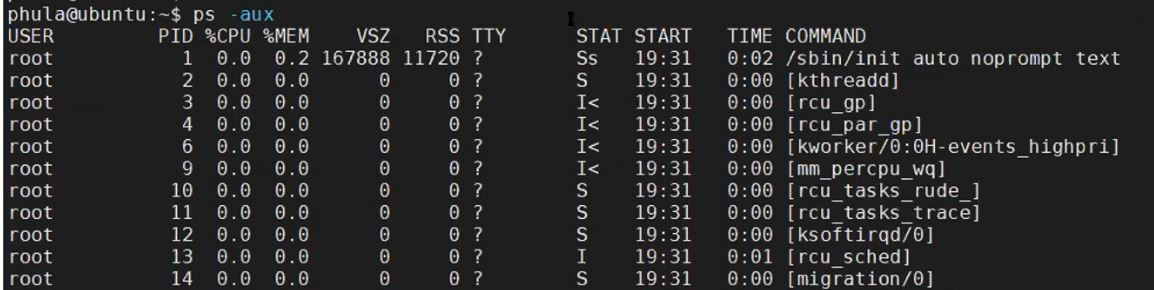
\includegraphics[scale=0.5]{emLinux_c03_fields-of_ps-aux_command}
  \caption{Fields of ps-aux command}  
\end{figure}
\\safe functions to run in the signal handler: slide 11 of 16 of signal ppt.
\\or the keywords: reentrant functions in linux
\\tat ca driver deu co process\_id = 0
\\search keyword 'passing arguments to signal handler' de tim hieu ve pass du lieu vao trong signal handler

\subsection{Vid 4 - Interrupt (Nov 15, 2021)}
tao 1 thread de doc du lieu ngay nay qua thang no.
\\khi nao thi deadlock xay ra
\\gg thread\_create in man7.org
\\sau khi dung lenh pthread\_create thi phai dung lenh pthread\_join
\\1h09m: khi chay nhieu thread, co the bi loi race\_condition
\\1h29m: lenh atomic trong c++, atomic\_increase(a);
\\1h39m: mutex in operating system: khoa 1 chia, mutex\_lock
\\semaphore la khoa nhieu chia
\\1h55m: wrapper function
\\task in RTOS is as same as process in Linux
\\truyen tin giua cac task thi giong voi co che chuyen tin cua process
\\dung lenh time ./mutex thi se in ra tgian chay doan code do.
\\build ra file lib de lam gi.
\\2h26m: end of video




\subsection{Vid 9 - Interrupt (Nov 13, 2021)}

How to connect ssh using the internet
\begin{itemize} 
  \item cam day mang vao cong internet cua beaglebone
  \item sudo apt-get install openssh-server
  \item Ben board beaglebone thi dung lenh sudo ifconfig de xem dia chi ip cua day internet eth0
  \item Tai may windows thi dung mobaXterm, va go lenh ssh debian@192.168.0.43.
  \item sudo \path{nano/etc/ssh/sshd_config}
\end{itemize}


\subsection{Vid 13 - Watchdog (Dec 04, 2021)}
Quy tac 5 buoc de viet driver
\begin{itemize}
  \item Tim hieu hardware 
  \item Tim hieu standard giao tiep giua OS va device file cua module do
  \item Tim hieu template driver
  \item Viet driver
\end{itemize}
scp my\_watchdog.ko debian@192.168.0.43: lenh de copy 1 file tu may ubuntu sang may BBB
\\dung lenh 'sudo su' de login o dang root, sau do
\\insmod my\_watchdo.ko sau moi lan reset
\\dung lenh \path{./main_test} de test watchdog
\\Dat log la dat nhu the nao

\subsection{Vid 14 - Uboot (Dec 11, 2021)}
Tai lieu tra cuu uboot - Uboot reference manual,
link \path{https://hub.digi.com/dp/path=/support/asset/u-boot-reference-manual/}\\
\\File uEnv.txt la cho de config cho uboot
\\Homework: sua lai tgian boot cua uboot, de tgian doi ng dung tu 1s tro thanh 30s. 
Co nhieu cach de sua, build lai uboot va ghi vao the.\\
\\Tra trong reference manual, uboot, page 15, bootdelay
\\Node trong Embedded linux la sao?
\\Buildroot vs Yocto, framework de build la gi. 
Buildroot ra doi truoc nhung Yocto ra doi sau nhung tot hon, tuy theo tinh nang
\\OTA update linux - Mender, co the update app va framework OTA
\\Homework 2: type 'hello Phu', show 'xin chao Phu'